\chapter{Introdução}
\label{cap:introducao}

Este capítulo apresenta os fundamentos contextuais, normativos e metodológicos que estruturam esta monografia. Inicialmente, expõem-se a evolução dos serviços públicos digitais no Brasil, a arquitetura tecnológica das infraestruturas governamentais investigadas e o arcabouço regulatório federal de segurança da informação e gestão de registros de auditoria. Na sequência, delimitam-se o problema técnico de pesquisa e a modelagem do objetivo conceitual, da questão de pesquisa principal e das métricas operacionais sob o paradigma \textit{Goal Question Metric} (GQM). Em seguida, estabelecem-se os objetivos geral e específicos e detalha-se a metodologia da pesquisa, fundamentada em um estudo de caso único incorporado apoiado por uma revisão estruturada da literatura. Por fim, descrevem-se a organização dos capítulos da monografia e o fluxo de atividades distribuído entre as duas etapas do Trabalho de Conclusão de Curso.

\section{Contexto}
\label{sec:intro_contexto}


A transformação digital do Estado brasileiro \textcolor{red}{consolidou as plataformas computacionais como o canal primário de mediação entre o poder público e a sociedade civil.}  \todo[color=yellow, size=\tiny]{Essa afirmação  é meio forte. A lei por si só não consolida nada. Talvez seja melhor dizer que a lei impulsionou a consolidação das plataformas computacionais como o canal primário de mediação entre o poder público e a sociedade civil.}
 Impulsionada pelas diretrizes de eficiência e governo digital da Lei nº 14.129/2021 \cite{lei14129_2021}, a oferta centralizada de serviços digitais na Administração Pública Federal ampliou o alcance das políticas públicas e a transparência institucional. Entretanto, auditoria operacional do Tribunal de Contas da União sobre fraudes e incidentes cibernéticos demonstrou que a digitalização massiva e a concentração de dados pessoais sob custódia estatal expandiram proporcionalmente a superfície de ataque das instituições públicas \cite{tcu_golpes2025}, exigindo controles rigorosos de proteção de dados nos termos da Lei Geral de Proteção de Dados Pessoais, Lei nº 13.709/2018 \cite{lgpd2018}.

No área da Engenharia de Software, a proteção de informações e a rastreabilidade de operações consolidaram-se como atributos essenciais de qualidade de produto e de processo. A norma ISO/IEC 25010:2023 posiciona a segurança como característica primária de qualidade do produto, com destaque para o não repúdio e a responsabilização como bases para a auditabilidade de eventos \cite{iso25010_2023}, enquanto a \cite{iso27001_2022} estabelece os requisitos de gestão da segurança da informação. Paralelamente, a sustentação de plataformas governamentais passou a apoiar-se em arquiteturas nativas em nuvem baseadas em contêineres orquestrados por Kubernetes e em ciclos contínuos de DevSecOps, impondo a automação da verificação de segurança e da observabilidade em tempo de execução \cite{fitzgerald2017,rajapakse2022}.
\todo[inline, color=pink]{Essa ultima frase tem um problema parecido. Essa referencia (fitzgerald2017) não diz o que a frase afirma. Nessa segunda (rajapakse2022) os autores dizem isso?}

Para disciplinar a governança cibernética nos órgãos integrantes do Sistema de Administração dos Recursos de Tecnologia da Informação (SISP), a Secretaria de Governo Digital instituiu o Programa de Privacidade e Segurança da Informação pela Portaria SGD/MGI nº 852/2023 \cite{portaria852_2023}, atualizado para a versão PPSI 2.0 pela Portaria SGD/MGI nº 9.511/2025 \cite{portaria9511_2025}. O Guia do arcabouçoz do PPSI 2.0 alinha seus controles técnicos ao catálogo internacional \textit{CIS Controls} na versão 8.1 \cite{ppsi2026,cis2024}, destacando o Controle 8, cujo propósito consiste em coletar, alertar, analisar e reter registros de auditoria capazes de detectar ataques cibernéticos e subsidiar a recuperação operacional. Para o ciclo de 2026, a Instrução Normativa SGD/MGI nº 4/2026 regulamentou a priorização das salvaguardas e formalizou os indicadores oficiais de maturidade para a avaliação de conformidade \cite{in4_2026}.

As diretrizes de governança do PPSI 2.0 articulam-se aos requisitos forenses da Norma Complementar nº 21/IN01/DSIC/GSI-PR, que exige a sincronização dos ativos com a Hora Legal Brasileira, o registro de eventos críticos acompanhado de metadados mínimos de identificação, a centralização remota e a guarda íntegra pelo prazo normativo mínimo de seis meses, sem prejuízo de prazos previstos em legislações específicas \cite{nc21_2014}. Em infraestruturas distribuídas em nuvem, o cumprimento dessas obrigações observa ainda o modelo de responsabilidade compartilhada disciplinado pela Instrução Normativa GSI/PR nº 5/2021 \cite{ingsi5_2021} e detalhado no Guia Complementar de Computação em Nuvem do PPSI 2.0 \cite{guianuvem2025}, segundo o qual compete ao órgão público gestor configurar, centralizar, reter e monitorar os registros de auditoria dos sistemas operacionais, das malhas de orquestração e das aplicações sob seu controle.

\section{Problema}
\label{sec:intro_problema}

Apesar da obrigatoriedade do arcabouço normativo federal, auditorias de controle externo evidenciam uma defasagem sistêmica na implementação de controles técnicos de segurança cibernética no Poder Executivo Federal. No Acórdão nº 2.387/2024 do Plenário do Tribunal de Contas da União \cite{tcu2387_2024}, que auditou 253 organizações integrantes do SISP, constatou-se baixa maturidade operacional e expediu-se ciência formal a 101 entidades federais que sequer haviam apresentado diagnósticos e planos de ação do PPSI.

Esse déficit torna-se particularmente sensível em infraestruturas de homologação e produção baseadas em contêineres, nas quais a natureza efêmera de \textcolor{red}{\textit{pods}} \todo[color=yellow, size=\tiny]{O que são pods?} e contêineres dificulta a preservação forense quando os registros são mantidos apenas localmente, pois a destruição do contêiner apaga as evidências antes de sua coleta e centralização \cite{jin2025,zhang2025}. Nesses ambientes, a ausência de monitoramento centralizado em tempo de execução oculta incidentes na cadeia de suprimentos de software, compromete a custódia probatória exigida pelos órgãos de controle externo \cite{tcu2387_2024,lgpd2018}. Soma-se à isso, a lacuna constatada na Revisão Estruturada da Literatura apresentada no Capítulo~\ref{cap:revisao_sistematica}, segundo a qual a maioria dos estudos da área não avalia o grau de conformidade inicial antes de intervir na infraestrutura.

Diante desse cenário técnico e regulatório, o problema de pesquisa que motiva esta investigação é formalmente enunciado nos seguintes termos: \textbf{a infraestrutura de homologação e produção de plataformas digitais governamentais federais carece de monitoramento de segurança centralizado em tempo de execução, contrariando as exigências do Controle 8 do PPSI 2.0 e da NC 21 do GSI-PR, conforme evidenciado no Acórdão nº 2.387/2024/TCU.} Essa lacuna expõe um vetor crítico na cadeia de suprimentos de software governamental que permanece sem uma avaliação do seu grau de conformidade em tempo de execução.

\section{Questão de Pesquisa}
\label{sec:intro_questao_pesquisa}

\subsection{GQM Adaptado}
\label{subsec:intro_gqm}

Para conectar o problema de pesquisa a critérios quantitativos e auditáveis de avaliação \cite{wohlin2024,runeson2009}, adotou-se o paradigma \textit{Goal Question Metric} (GQM), proposto por \citeonline{basili1994}, adaptado para o contexto da pesquisa. Essa abordagem estrutura o programa de medição de forma descendente em três níveis integrados: o nível conceitual, que especifica o objetivo de medição em função do objeto de estudo, do propósito, do foco de qualidade, do ponto de vista e do contexto; o nível operacional, composto pela questão de pesquisa que deriva do objetivo e caracteriza o objeto sob investigação; e o nível quantitativo, constituído pelas métricas associadas para responder à questão de forma objetiva \cite{basili1994}, conforme ilustrado na Figura~\ref{fig:intro_gqm}.

\begin{figure}[H]
    \centering
    \caption{Estrutura hierárquica da abordagem GQM}
    \label{fig:intro_gqm}
    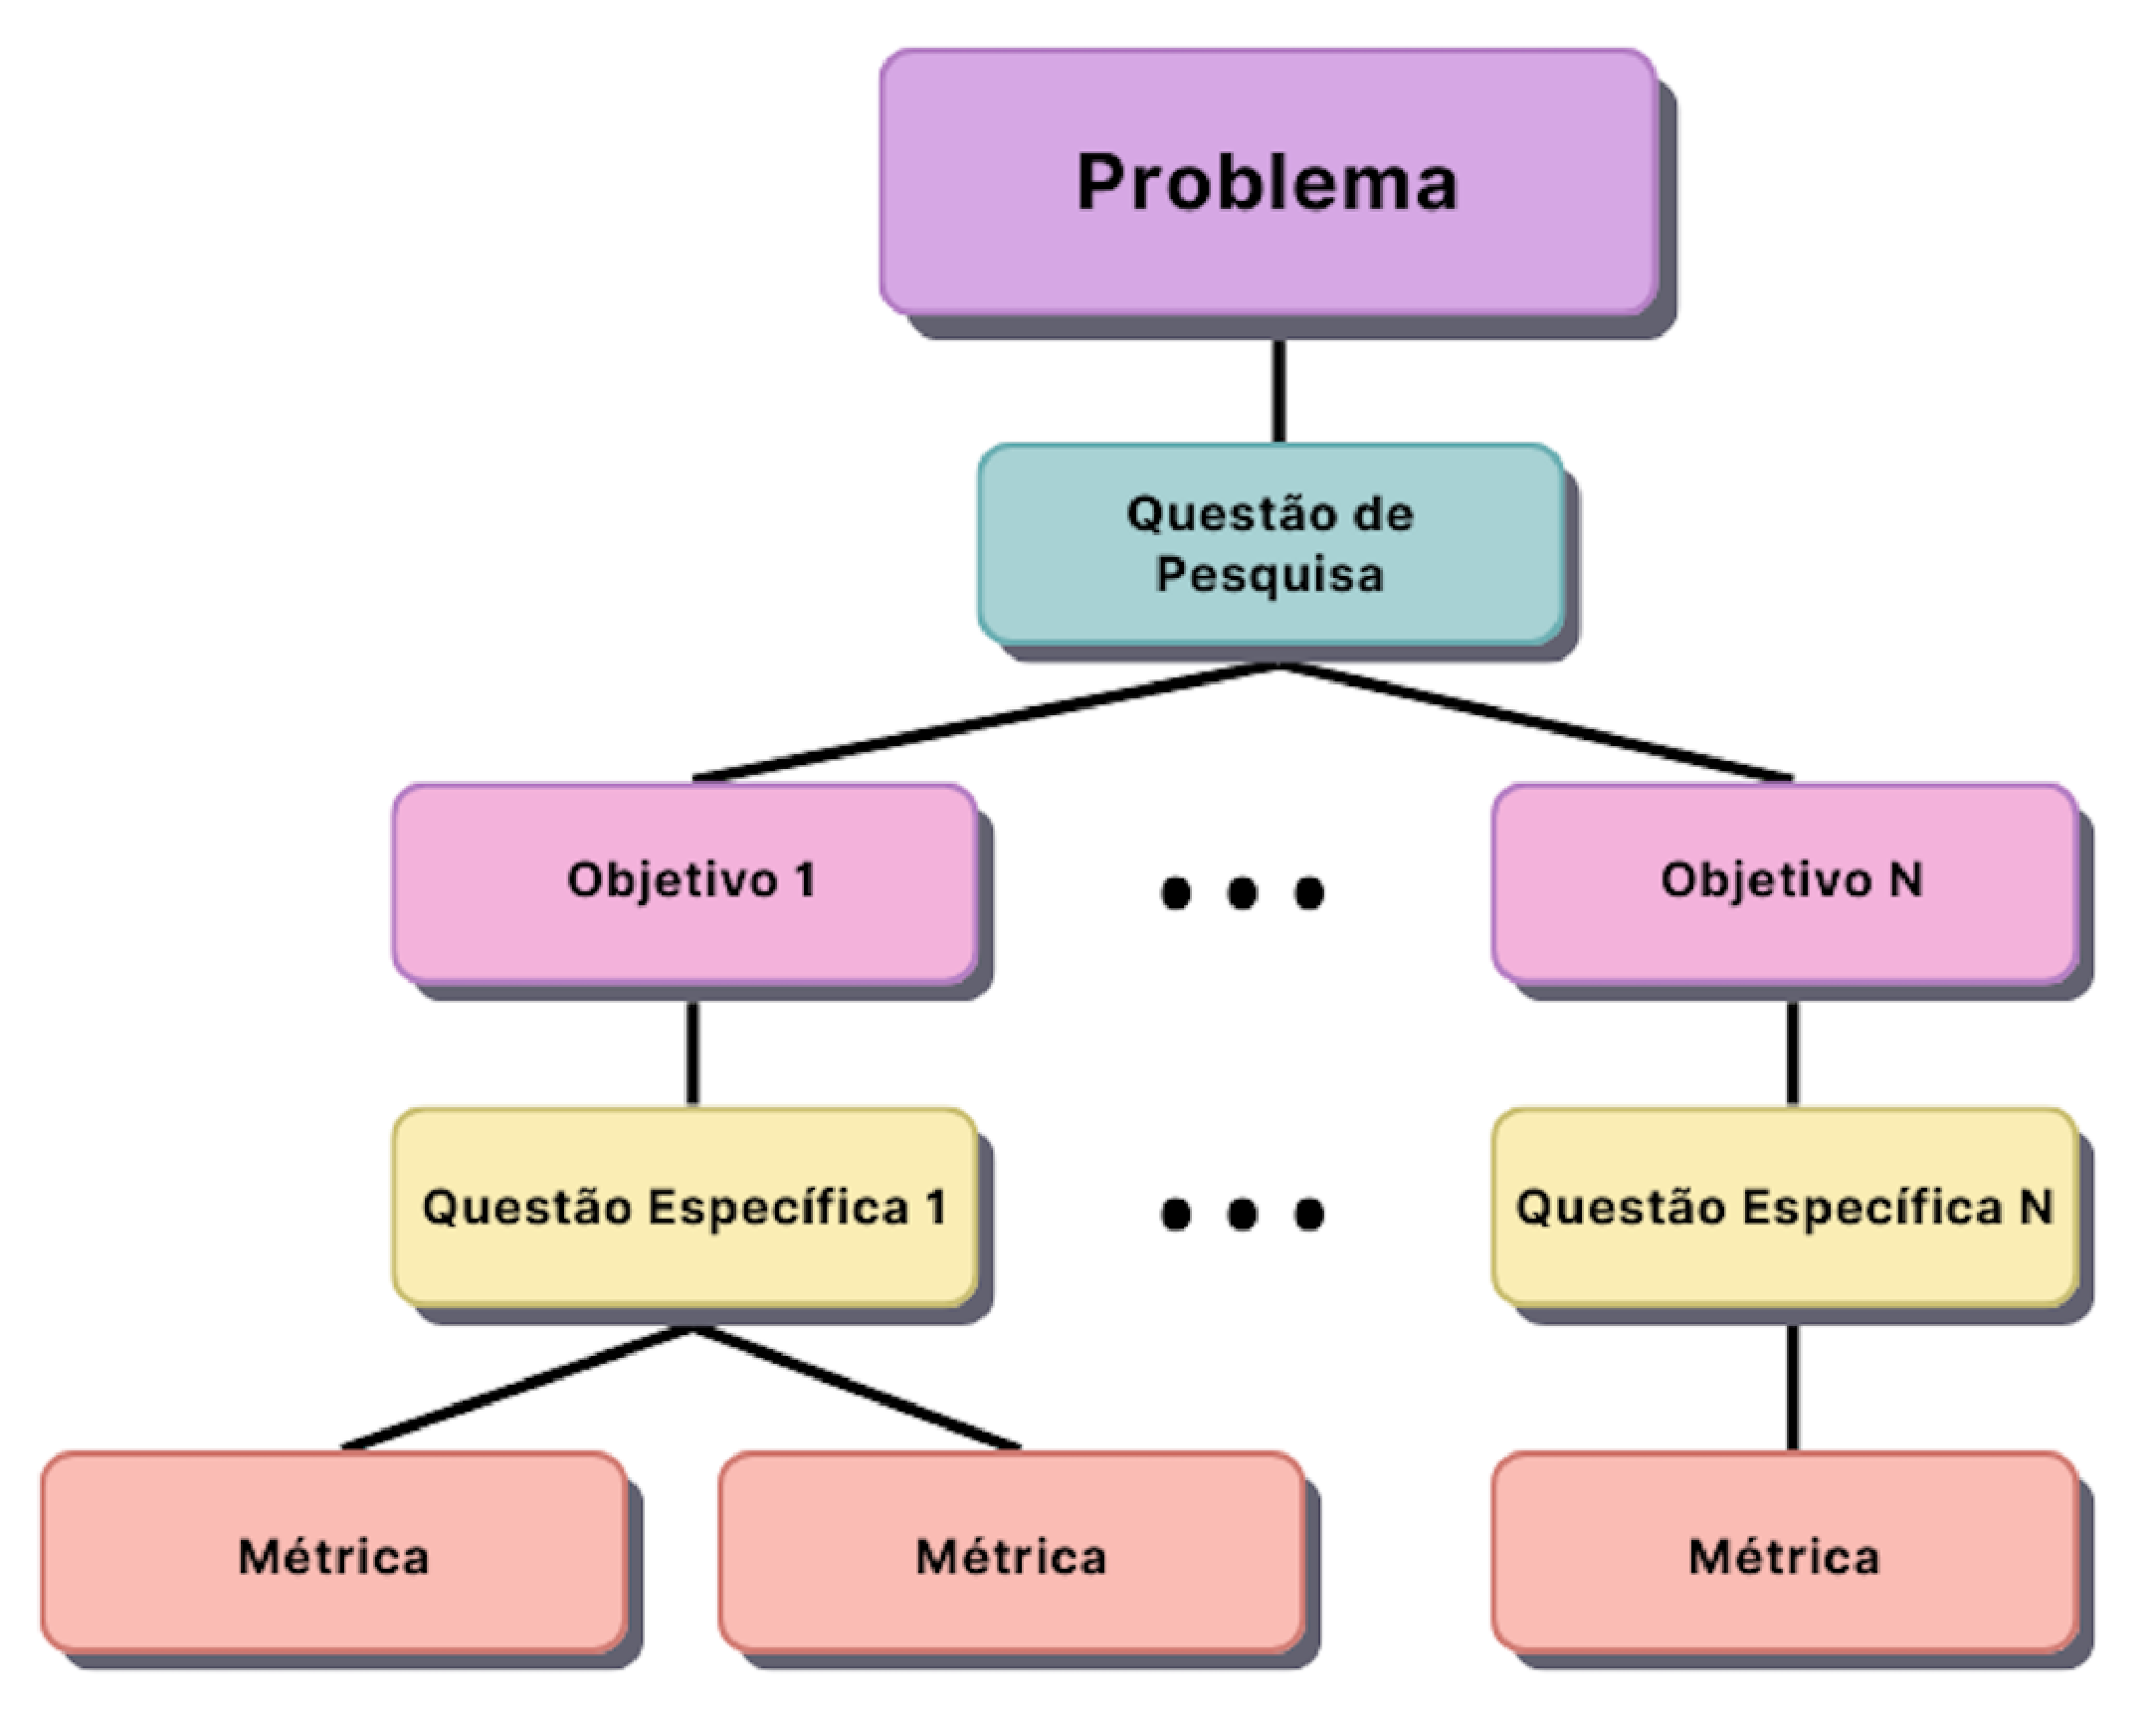
\includegraphics[width=0.5\textwidth]{figuras/gqm.eps}
    \fonte{Adaptado de \citeonline{basili1994}.}
\end{figure}

Segundo as cinco dimensões estabelecidas por \citeonline{basili1994}, a Tabela~\ref{tab:intro_gqm_objetivo} apresenta a decomposição estruturada do objetivo conceitual de medição desta pesquisa ao que se chama de GQM adaptado.

\begin{table}[H]
    \centering
    \caption{Definição do objetivo conceitual de medição segundo o paradigma GQM}
    \label{tab:intro_gqm_objetivo}
    \small
    \begin{tabular}{p{4.6cm}p{9.8cm}}
        \hline
        \textbf{Parâmetro GQM} & \textbf{Definição no Estudo} \\ \hline
        \textbf{Analisar} (\textit{Object of Study}) & A infraestrutura de monitoramento de segurança cibernética em tempo de execução de sistemas digitais da Administração Pública Federal. \\ \hline
        \textbf{Com o propósito de} (\textit{Purpose}) & Avaliar o grau de conformidade perante o normativo nacional. \\ \hline
        \textbf{Com respeito ao} (\textit{Focus}) & Grau de aderência técnica às 12 medidas do Controle 8 do PPSI 2.0 e aos requisitos da NC 21 do GSI-PR. \\ \hline
        \textbf{Do ponto de vista do} (\textit{Point of View}) & Pesquisador. \\ \hline
        \textbf{No contexto do} (\textit{Context}) & Infraestrutura de homologação e produção orquestrada por Kubernetes de plataformas digitais da Administração Pública Federal sujeitas às diretrizes de conformidade do PPSI 2.0. \\ \hline
    \end{tabular}
    \fonte{Elaborado pelo Autor}
\end{table}




No nível operacional, a estrutura conceitual definida no GQM adaptado é diretamente transformada na questão de pesquisa principal que norteia este trabalho:

\textbf{Como avaliar, em tempo de execução, o grau de conformidade da infraestrutura de monitoramento de segurança cibernética dos sistemas digitais da Administração Pública Federal segundo o Controle 8 do PPSI 2.0 e com os requisitos da NC 21 do GSI-PR?}

Para responder a essa questão norteadora com rigor metodológico, a pesquisa desdobra-se em dois estudos empíricos complementares: uma Revisão Estruturada da Literatura, orientada por doze questões secundárias específicas, para conhecermos como o tema de pesquisa deste trabalho é abordado na literatura científica, com vistas a identificar lacunas de pesquisa e subsidiar o planejamento do estudo de caso, voltado a diagnosticar e avaliar empiricamente a infraestrutura computacionalde uma entidade da Administração Pública Federal.

No nível quantitativo, a operacionalização da avaliação adota os critérios oficiais estabelecidos pela Instrução Normativa SGD/MGI nº 4/2026 \cite{in4_2026}. A pesquisa utiliza o Nível de Implementação da Medida (NIM) para avaliar o atendimento individual de cada salvaguarda do Controle 8 em uma escala ordinal de zero a cinco, e o Nível de Adoção do Controle (NAC), que expressa a maturidade global do ambiente por meio da média aritmética dos índices aplicáveis aferidos.

\section{Objetivos}
\label{sec:intro_objetivos}

Os objetivos desta monografia foram delineados em alinhamento direto com o objetivo conceitual do modelo GQM e com a questão de pesquisa estabelecida, dividindo-se em objetivo geral e objetivos específicos.

\subsection{Objetivo Geral}
\label{subsec:intro_objetivo_geral}
\label{subsec:intro_obj_geral}

O objetivo geral desta pesquisa consiste em executar a avaliação  descrita no nível conceitual do GQM, conforme a Seção~\ref{subsec:intro_gqm}, aferindo o grau de conformidade técnica da infraestrutura estudada de acordo com o Controle 8 do PPSI 2.0 e a NC 21 do GSI-PR.

\subsection{Objetivos Específicos}
\label{subsec:intro_objetivos_especificos}
\label{subsec:intro_obj_especificos}

Para alcançar o objetivo geral proposto, foram definidos os seguintes objetivos específicos:
\begin{itemize}
    \item Fundamentar os conceitos de Engenharia de Software Experimental, qualidade e segurança de software, orquestração de contêineres em Kubernetes, plataformas SIEM e HIDS e o arcabouço normativo federal composto pelo PPSI 2.0, CIS Control 8, IN SGD/MGI nº 4/2026 e NC nº 21/IN01/DSIC/GSI-PR;
    \item Conduzir uma Revisão Estruturada da Literatura, baseada no protocolo de \citeonline{kitchenham2007}, sobre soluções de monitoramento de segurança em tempo de execução, gestão centralizada de registros \textit{logs} de auditoria e avaliação de conformidade normativa em ambientes distribuídos e em nuvem;
    \item Estruturar uma matriz de evidências técnicas para operacionalizar as métricas de Nível de Implementação da Medida (NIM) e Nível de Adoção do Controle (NAC), em conformidade com os critérios da IN SGD/MGI nº 4/2026;
    \item Planejar um estudo de caso único incorporado segundo as diretrizes de \citeonline{runeson2009} e \citeonline{yin2015}, delimitando o contexto da infraestrutura Kubernetes, as unidades de análise e os procedimentos de coleta e análise de dados;
    \item Planejar e estabelecer os critérios para o diagnóstico inicial de linha de base de conformidade da infraestrutura; e
    \item Propor uma arquitetura de monitoramento e auditoria de segurança em tempo de execução baseada na integração entre configurações nativas de auditoria e registro do Kubernetes, abrangendo plano de controle, nós e serviços internos, e a coleta, normalização, correlação e retenção centralizada pelo SIEM Wazuh, com vistas a elevar o Nível de Adoção do Controle 8 do PPSI 2.0 e o atendimento aos requisitos forenses da NC nº 21/GSI-PR, a ser implementada na segunda etapa da pesquisa.
\end{itemize}

\section{Metodologia}
\label{sec:intro_metodologia}

O delineamento metodológico desta investigação fundamenta-se na taxonomia de pesquisa em Engenharia de Software Experimental \cite{wohlin2024} e nas diretrizes específicas para condução de Estudos de Caso nessa área \cite{runeson2009,yin2015}, organizando-se nas fases estratégica, tática e operacional, conforme representado na Figura~\ref{fig:intro_metodologia_fluxo}.

Na \textbf{fase estratégica}, que parte da questão de pesquisa formulada, a investigação classifica-se quanto ao resultado como uma \textbf{Pesquisa Aplicada}, voltada a solucionar um problema concreto de aferição de conformidade normativa e visibilidade de segurança cibernética em infraestruturas governamentais reais. Quanto à lógica de investigação, adota-se uma abordagem \textbf{Indutiva}, partindo  de premissas normativas formais do PPSI 2.0, do Controle 8 do CIS e da NC nº 21/GSI-PR, estruturadas pelo modelo GQM, em combinação com a análise das evidências empíricas levantadas na literatura e no ambiente operacional. Quanto ao propósito, o estudo apresenta natureza \textbf{ Avaliativa}, visto que explora o estado da arte em telemetria de segurança em tempo de execução, descreve a arquitetura e as lacunas de auditoria da infraestrutura sob estudo e avalia objetivamente seu grau de aderência regulatória \cite{wohlin2024,runeson2009}. Quanto ao paradigma, a pesquisa alinha-se à perspectiva \textbf{Positivista}, \textcolor{red}{É intrepretativista/costrutivista} \todo[color=yellow, size=\tiny]{É o oposto do positivismo. Reescrever.} apoiando-se em proposições estruturadas, critérios de evidência previamente definidos e medições independentes de subjetividade do observador \cite{runeson2009}. 

Na \textbf{fase tática}, o processo de pesquisa adota uma \textbf{Abordagem Mista}, articulando dados qualitativos provenientes do exame de artefatos arquiteturais, manifestos de configuração e requisitos forenses com dados quantitativos expressos pelos indicadores NIM e NAC \cite{runeson2009}. Como metodologia central, emprega-se um \textbf{Estudo de Caso Único Incorporado} \cite{runeson2009,yin2015}. O caso holístico corresponde à infraestrutura de orquestração de contêineres Kubernetes mantida pelo laboratório de pesquisa e inovação em software da Universidade de Brasília, LabLivre/LAPP1S. Como a Universidade de Brasília integra a Administração Pública Federal e o laboratório opera ambientes próprios de homologação e produção, além de hospedar plataformas digitais governamentais como por exemplo, o \textcolor{red}{GovHub} \todo[color=yellow, size=\tiny]{Inserir nota de rodapé com a url de acesso}  e o   \textcolor{red}{Brasil Participativo,} \todo[color=yellow, size=\tiny]{Inserir nota de rodapé com a url de acesso} essa infraestrutura submete-se diretamente às exigências do PPSI 2.0 e da NC nº 21/GSI-PR. O recorte incorporado desdobra o caso em múltiplas subunidades de análise, formadas pelos artefatos declarativos de configuração, pelos registros em tempo de execução e pelos eventos e relatórios consolidados no SIEM, avaliados contra as doze salvaguardas previstas no Controle 8 do PPSI 2.0 e os requisitos da NC nº 21/GSI-PR conforme detalhado no Capítulo~\ref{cap:estudo_de_caso}.

\todo[inline, color=pink]{Alguns itens da metodologia eu corrigi direto no texto, mas outros eu deixei para você corrigir. Holístico e incorporado são alternativas excludentes e o seu estudo é incorporado.}

\todo[inline, color=pink]{1)O que você chama de subunidades são fontes de dados, não unidades de análise. Defina como unidades de análise os componentes da infraestrutura de monitoramento: plano de controle, nós hospedeiros, cargas de trabalho, serviços de rede do cluster (se avaliados) e SIEM. 
2)Os artefatos (configurações, registros brutos, eventos do SIEM) são fontes de evidência coletadas em cada unidade. 
3) As doze salvaguardas são os critérios de avaliação. As salvaguardas de processo são avaliadas no nível do caso. 
4)Corrija a descrição do ambiente (existe apenas homologação), refaça a justificativa de aplicabilidade das normas para esse ambiente e declare como limitação que os registros de homologação não representam carga de produção.}



Na \textbf{fase operacional}, os procedimentos de coleta de dados combinam dois métodos complementares:
\begin{itemize}
    \item \textbf{Revisão Estruturada da Literatura:} conduzida na primeira etapa mediante o protocolo de revisão sistemática de \citeonline{kitchenham2007} para mapear ferramentas de monitoramento em tempo de execução, técnicas de coleta de registros e modelos de avaliação de conformidade; e
    \item \textbf{Análise Documental e de Artefatos:} empregada na inspeção dos normativos federais vigentes e na extração não intrusiva de manifestos, configurações e registros de auditoria na linha de base e no cenário pós-intervenção \cite{runeson2009,wazuh2025}.
\end{itemize}

Por fim, o processamento e a interpretação dos dados obtidos apoiam-se em dois métodos analíticos:

\todo[inline, color=pink]{Você não fará análise temática e de conteúdo, mas sim, análise de conteúdo, que é um método de análise qualitativa mais abrangente. Análise temática utiliza  técnica distinta.}

\begin{itemize}
    \item \textbf{Análise Temática e de Conteúdo:} utilizada para categorizar qualitativamente os artefatos coletados frente aos requisitos normativos do Controle 8 do PPSI 2.0 e da NC nº 21/GSI-PR; e
    \item \textbf{Mensuração Quantitativa Determinística:} empregada no cálculo aritmético direto das fórmulas estabelecidas pela IN SGD/MGI nº 4/2026 para apurar os indicadores oficiais NIM e NAC.
\end{itemize}

\begin{figure}[htbp]
    \centering
    \caption{Taxonomia e delineamento metodológico da pesquisa}
    \label{fig:intro_metodologia_fluxo}
    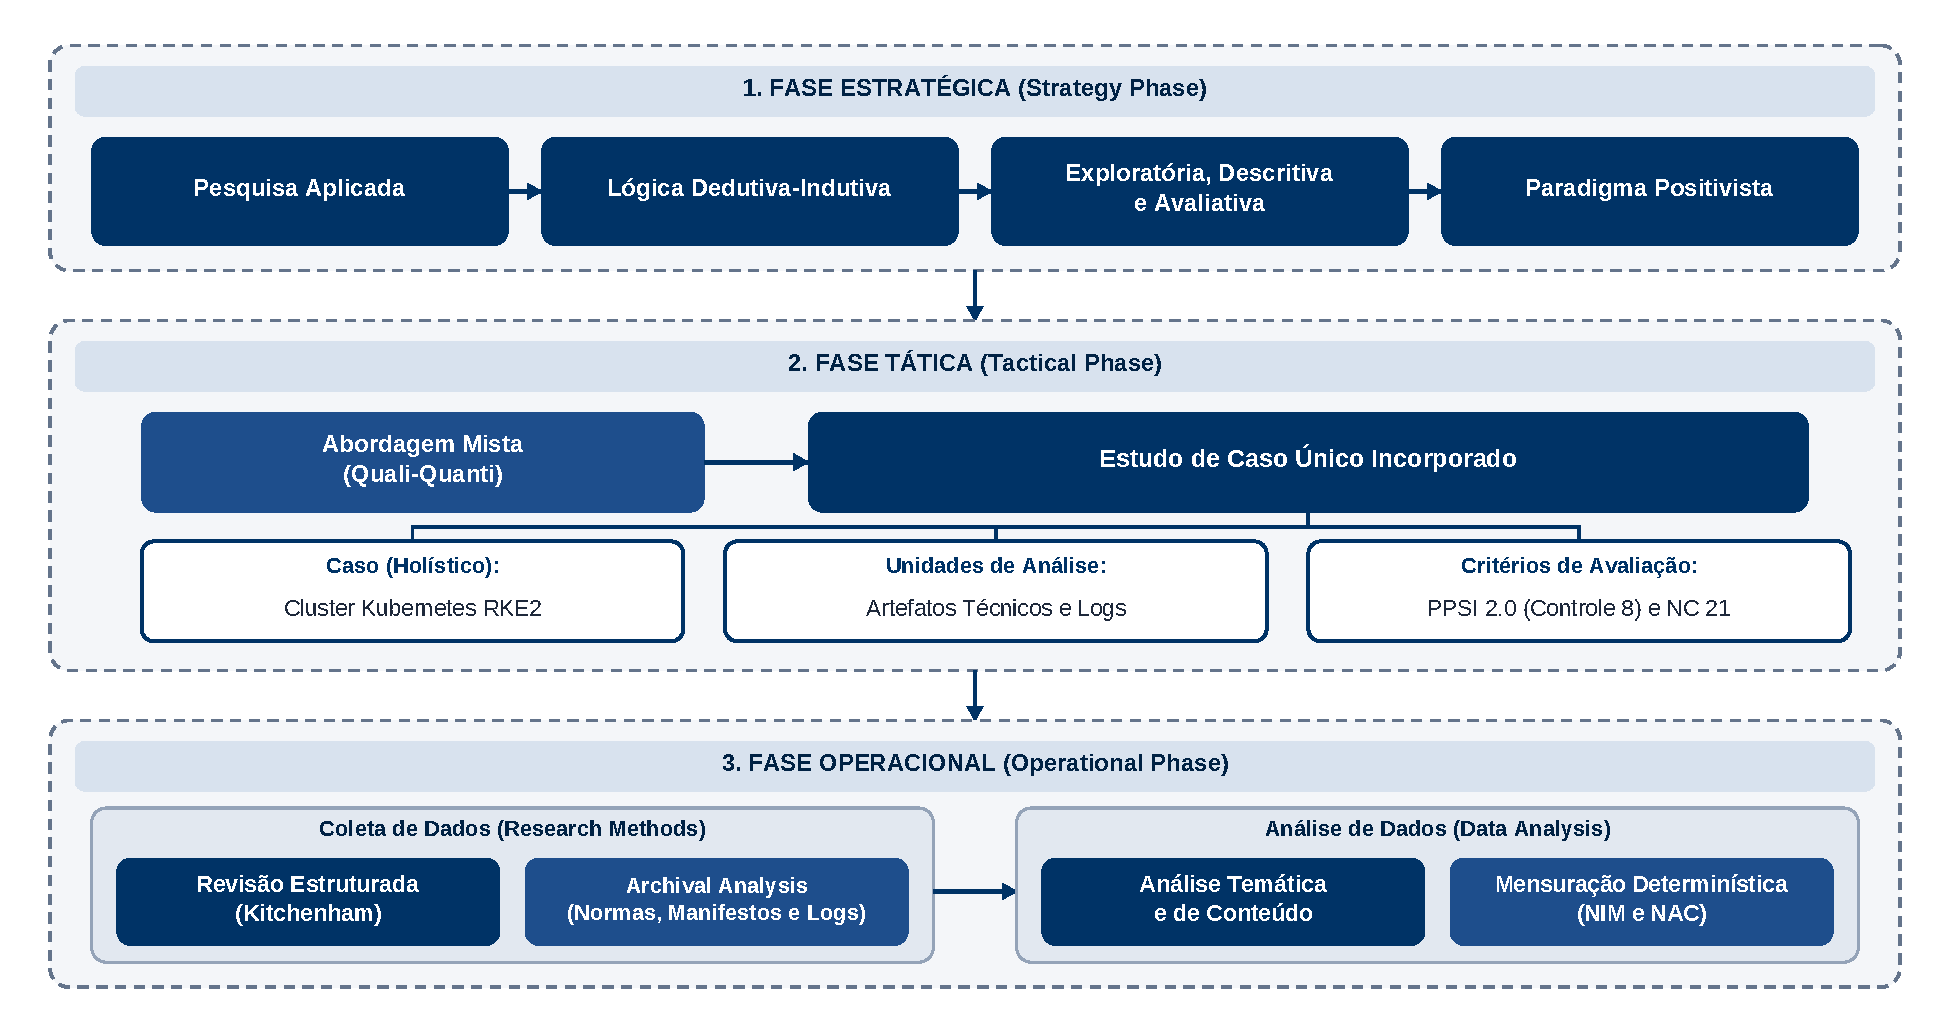
\includegraphics[width=0.98\textwidth]{figuras/fluxo_metodologia.eps}
    \fonte{Adaptado pelo autor.}
\end{figure}


\todo[inline, color=pink]{Acertar a fig. 2 em função das correções sugeridas.}

\todo[inline, color=pink]{Sugiro você reler a teoria do cap. 2 do livro do wohlin. Ele fala sobre a diferença entre pesquisa aplicada e pesquisa básica, e também sobre a diferença entre pesquisa indutiva e dedutiva.}

\todo[inline, color=pink]{Caso Único ou Multiplos casos não foi discutido e você precisa justificar a escolha do caso único incorporado.}

\section{Organização do Trabalho}
\label{sec:intro_organizacao}

A estrutura desta monografia reflete o encadeamento lógico da metodologia científica adotada, distribuindo-se nos seguintes capítulos:
\begin{itemize}
    \item \textbf{Capítulo 1 -- Introdução:} apresenta a contextualização tecnológica e normativa da pesquisa, a definição do problema, a modelagem GQM e a questão de pesquisa principal, os objetivos geral e específicos, o delineamento metodológico, a organização do documento e o cronograma de atividades;
    \item \textbf{Capítulo 2 -- Referencial Teórico:} fundamenta os pilares conceituais e regulatórios do trabalho, abrangendo a Engenharia de Software Experimental com ênfase em Estudos de Caso, qualidade e segurança de software, arquiteturas nativas em nuvem e Kubernetes, monitoramento de segurança em \textit{runtime} via plataformas SIEM e HIDS e o detalhamento do PPSI 2.0, do Controle 8 do CIS, da IN SGD/MGI nº 4/2026 e da NC nº 21/GSI-PR;
    \item \textbf{Capítulo 3 -- Revisão Estruturada da Literatura:} documenta o protocolo de revisão fundamentado em \citeonline{kitchenham2007}, a estratégia de busca sob o modelo PIO, a triagem PRISMA, a síntese analítica dos estudos selecionados perante as doze questões secundárias de pesquisa, as lacunas identificadas na literatura e as ameaças à validade; e
    \item \textbf{Capítulo 4 -- Planejamento do Estudo de Caso:} formaliza o planejamento do estudo de caso único incorporado segundo as diretrizes de \citeonline{runeson2009} e \citeonline{yin2015}, caracteriza o contexto institucional e arquitetural da infraestrutura Kubernetes investigada, apresenta a questão de pesquisa do estudo de caso, define as unidades de análise, a operacionalização das métricas NIM e NAC e o protocolo de avaliação da linha de base e pós-intervenção a ser conduzido na segunda etapa.
    


\end{itemize}

\section{Cronograma e Fluxo de Atividades}
\label{sec:intro_cronograma}

O desenvolvimento completo desta pesquisa divide-se em duas etapas semestrais consecutivas, correspondentes às disciplinas de Trabalho de Conclusão de Curso 1 e Trabalho de Conclusão de Curso 2 da Faculdade UnB Gama. Nas subseções a seguir, discriminam-se o fluxo de atividades e o cronograma de cada etapa.

\subsection{Atividades da Primeira Etapa}
\label{subsec:intro_primeira_etapa}
\label{subsec:intro_etapa1}

Esta subseção discrimina as atividades executadas na primeira etapa da monografia, apresentando o encadeamento metodológico na Figura~\ref{fig:intro_fluxo_etapa1} e a distribuição cronológica na Figura~\ref{fig:intro_cronograma_etapa1}:
\begin{itemize}
    \item \textbf{Contextualização em ES Experimental:} estudo de revisões sistemáticas e estudos de caso em Engenharia de Software \cite{wohlin2024,runeson2009,yin2015};
    \item \textbf{Levantamento Normativo:} análise das diretrizes do PPSI 2.0, Controle 8 do CIS, IN SGD/MGI nº 4/2026, NC nº 21/GSI-PR e Acórdão nº 2.387/2024 -- TCU;
    \item \textbf{Definição do Problema e Modelo GQM:} formulação do problema, objetivo conceitual GQM \cite{basili1994}, questão principal e métricas NIM e NAC;
    \item \textbf{Elaboração do Protocolo de Revisão:} definição do protocolo segundo \citeonline{kitchenham2007}, modelo PIO, questões secundárias e \textit{string} de busca;
    \item \textbf{Triagem e Seleção dos Artigos:} execução da busca e filtragem auditável segundo o fluxo PRISMA na plataforma \textit{Evidentia};
    \item \textbf{Extração e Análise da Literatura:} leitura integral dos estudos selecionados, extração de dados e síntese das lacunas de pesquisa;
    \item \textbf{Planejamento do Estudo de Caso:} definição das unidades de análise, do protocolo de linha de base e da arquitetura proposta segundo \citeonline{runeson2009} e \citeonline{yin2015}; e
    \item \textbf{Redação, Revisão e Defesa do TCC 1:} redação dos capítulos da primeira etapa, revisões junto ao orientador e apresentação à banca examinadora.
\end{itemize}

\todo[inline, color=pink]{Retirar a fig. 3. As atividades não foram sequenciais, mas sim iterativas. A figura 4 é suficiente para mostrar o cronograma.}


\begin{figure}[htbp]
    \centering
    \caption{Fluxo de atividades da primeira etapa}
    \label{fig:intro_fluxo_etapa1}
    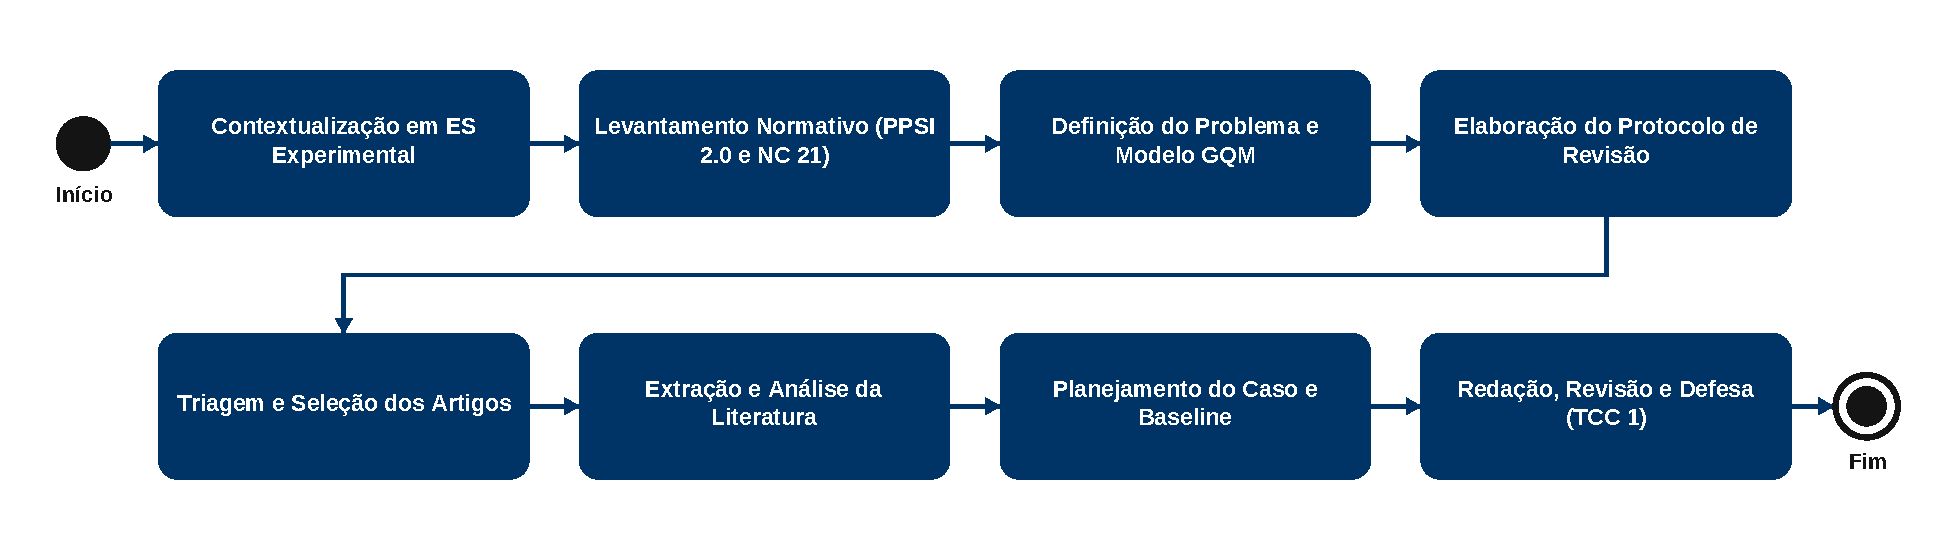
\includegraphics[width=0.94\textwidth]{figuras/fluxo_etapa1.eps}
    \fonte{Elaborado pelo autor.}
\end{figure}

\begin{figure}[htbp]
    \centering
    \caption{Cronograma da primeira etapa}
    \label{fig:intro_cronograma_etapa1}
    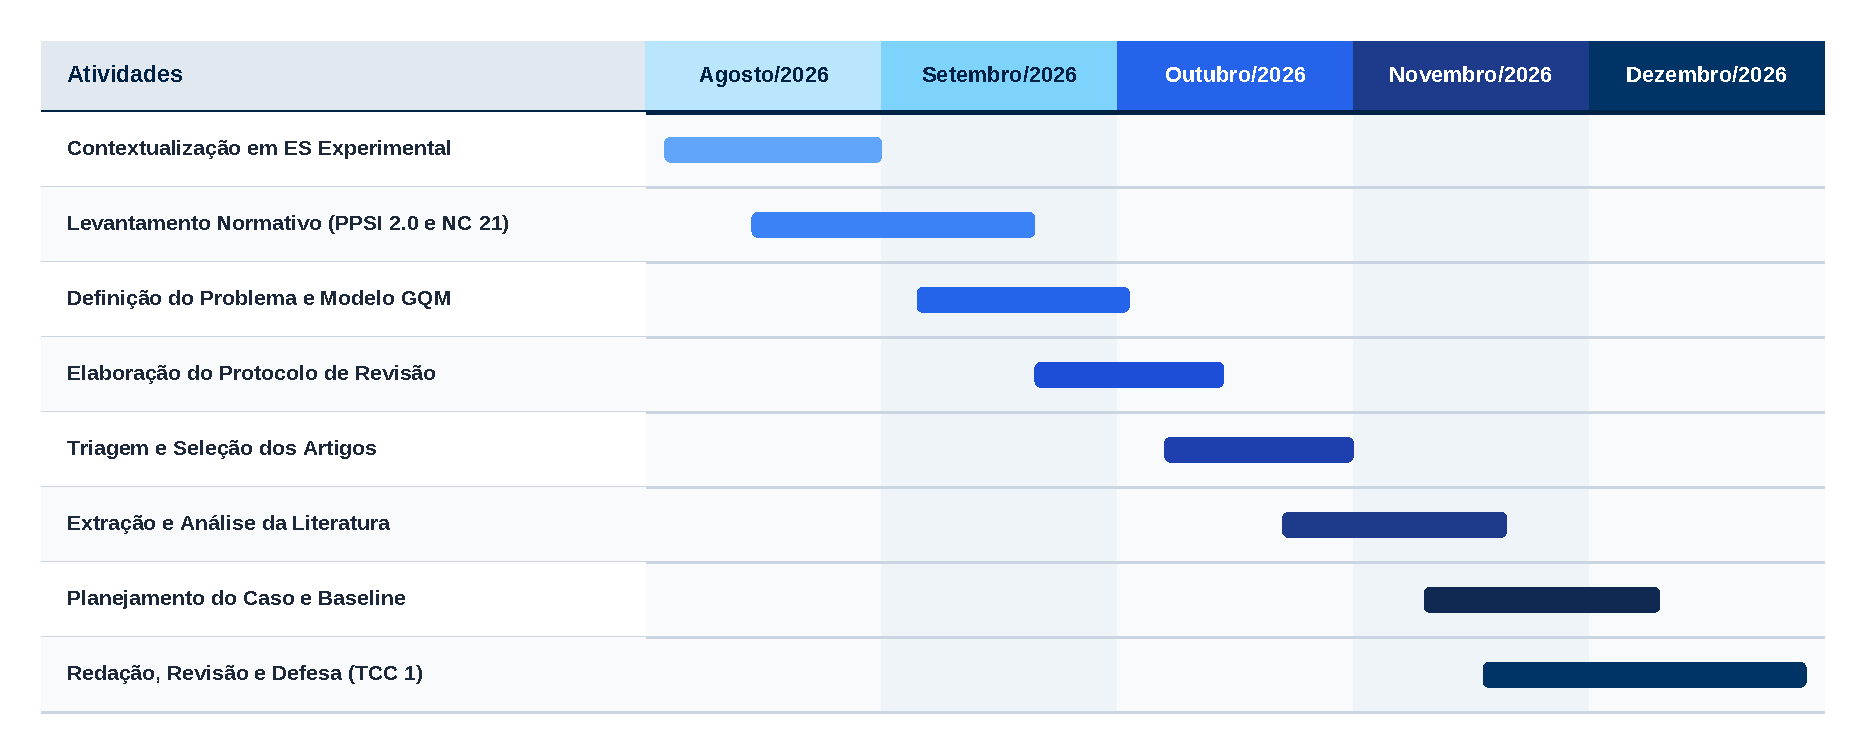
\includegraphics[width=0.94\textwidth]{figuras/cronograma_etapa1.eps}
    \fonte{Elaborado pelo autor.}
\end{figure}

\subsection{Atividades da Segunda Etapa}
\label{subsec:intro_segunda_etapa}
\label{subsec:intro_etapa2}

Esta subseção apresenta as atividades planejadas para a segunda etapa da pesquisa, cujo fluxo de execução e cronograma previsto encontram-se representados na Figura~\ref{fig:intro_fluxo_etapa2} e na Figura~\ref{fig:intro_cronograma_etapa2}, respectivamente:
\begin{itemize}
    \item \textbf{Refinamento Pós-Banca:} incorporação das recomendações metodológicas e técnicas apontadas pela banca na defesa da primeira etapa;
    \item \textbf{Execução do Diagnóstico Inicial (\textit{Baseline}):} coleta das evidências iniciais e apuração dos indicadores NIM e NAC antes da intervenção conforme o Capítulo~\ref{cap:estudo_de_caso};
    \item \textbf{Implantação do SIEM:} provisionamento da plataforma de SIEM Wazuh e distribuição dos agentes nos nós do \textit{cluster} Kubernetes \cite{wazuh2025};
    \item \textbf{Auditoria no Plano de Controle K8s:} ativação de políticas de auditoria nativas no plano de controle Kubernetes e de rastreamento nos nós hospedeiros;
    \item \textbf{Pareamento e Ingestão de Serviços:} integração dos registros nativos com decodificadores e regras customizadas no SIEM conforme a NC nº 21/GSI-PR;
    \item \textbf{Coleta em \textit{Runtime} e Aferição de Métricas:} extração dos artefatos pós-intervenção e cálculo determinístico dos indicadores NIM e NAC segundo a IN SGD/MGI nº 4/2026;
    \item \textbf{Análise Comparativa entre Linha de Base e Cenário Final:} cotejamento dos resultados para mensurar a evolução do NAC e discutir ameaças à validade; e
    \item \textbf{Redação, Revisão e Defesa Final:} consolidação dos resultados e conclusões da monografia, revisão final e defesa pública do TCC 2.
\end{itemize}

\begin{figure}[htbp]
    \centering
    \caption{Fluxo de atividades da segunda etapa}
    \label{fig:intro_fluxo_etapa2}
    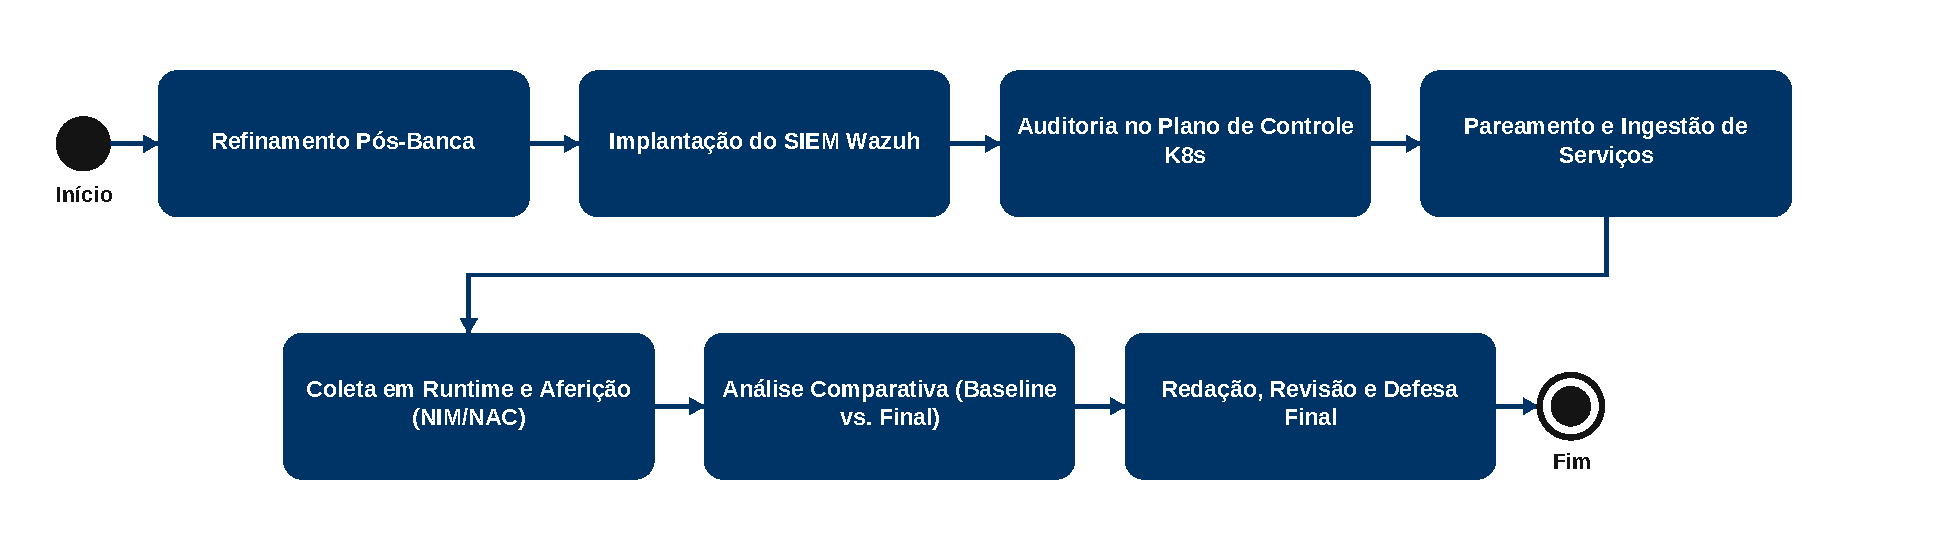
\includegraphics[width=0.94\textwidth]{figuras/fluxo_etapa2.eps}
    \fonte{Elaborado pelo autor.}
\end{figure}



\todo[inline, color=pink]{Retirar a fig. 5. As mesmas questões do comentário anterior. A figura 6 é suficiente para mostrar o cronograma.}







\begin{figure}[htbp]
    \centering
    \caption{Cronograma da segunda etapa}
    \label{fig:intro_cronograma_etapa2}
    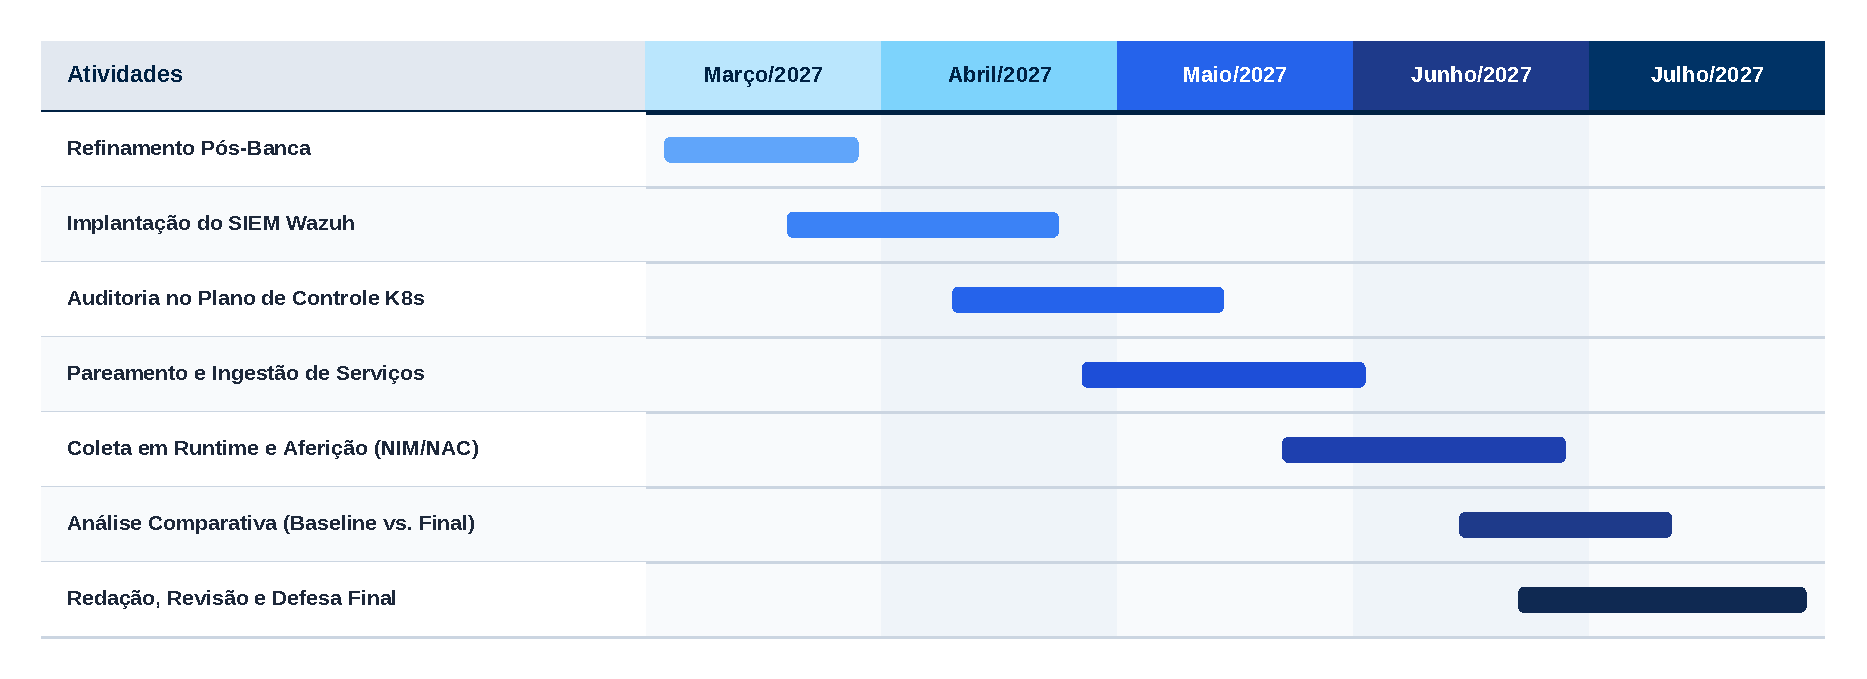
\includegraphics[width=0.94\textwidth]{figuras/cronograma_etapa2.eps}
    \fonte{Elaborado pelo autor.}
\end{figure}



\todo[inline, color=pink]{Embora você tenha herdado esse problema do template latex da unb, você precisa corrigir o problema de inserir uma página em branco entre os capítulos.}

